%  !TeX  root  =  user_guide.tex

\section{Labeling Plugin}

% when the revision of a section has been finalized,
% comment out the following line:
%\updatedisclaimer

The \toolbtntwo{labeling}{Labeling} plugin provides smart labeling for vector point, 
line and polygon layers and only requires a few parameters. This plugin will replace 
the current QGIS labeling and also supports on-the-fly transformated layers.

\begin{enumerate}
  \item Start QGIS and load a vector point, line or polygon layer. 
  \item Load the labeling plugin in the Plugin Manager (see Section 
  \ref{sec:load_core_plugin}), activate the layer in the legend and click on the 
  \toolbtntwo{labeling}{Labeling} icon which appears in the QGIS toolbar menu.
\end{enumerate}

\minisec{Labeling point layers}

First step is to activate the \checkbox{Label this layer} checkbox and select an attribute 
column to use for labeling. After that you can define the label placement and text style, 
labeling priority, scale-based visibility, if every part of multipart feature is to be 
labeled and if features act as obstacles for labels or not (see Figure \ref{fig:pointlabel}).  

\begin{figure}[ht]
\begin{center}
   \caption{Smart labeling of vector point layers \nixcaption}\label{fig:pointlabel}\smallskip
   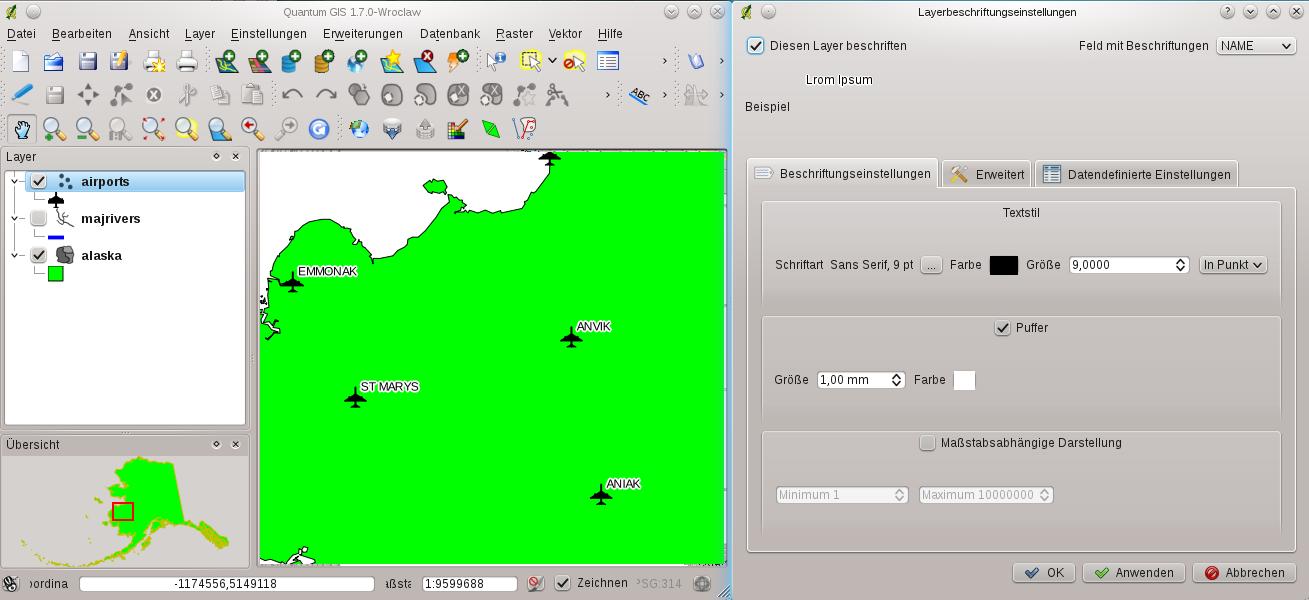
\includegraphics[clip=true, width=12cm]{label_points}
\end{center}
\end{figure}

\minisec{Labeling line layers}

First step is to activate the \checkbox{Label this layer} checkbox and select an attribute
column to use for labeling. After that you can define the label placement, orientation, 
distance to feature, text style, labeling priority, scale-based visibility, if every part 
of a multipart line is to be labeled, if lines shall be merged to avoid duplicate labels 
and if features act as obstacles for labels or not (see Figure \ref{fig:linelabel}).

\begin{figure}[ht]
\begin{center}
   \caption{Smart labeling of vector line layers \nixcaption}\label{fig:linelabel}\smallskip
   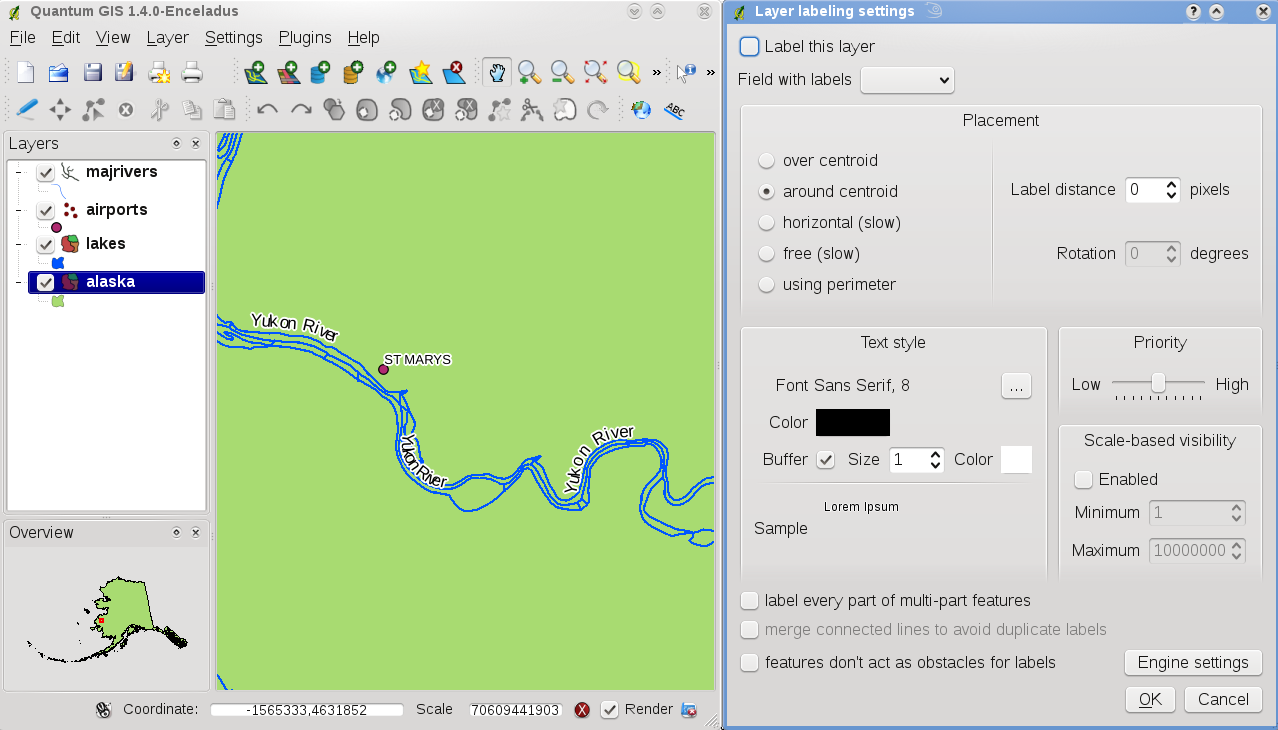
\includegraphics[clip=true, width=12cm]{label_line}
\end{center}
\end{figure}

\minisec{Labeling polygon layers}

First step is to activate the \checkbox{Label this layer} checkbox and select an attribute
column to use for labeling. After that you can define the label placement, distance and text 
style, labeling priority, scale-based visibility, if every part of multipart feature is to be
labeled and if features act as obstacles for labels or not (see Figure \ref{fig:arealabel}).

\begin{figure}[ht]
\begin{center}
   \caption{Smart labeling of vector polygon layers \nixcaption}\label{fig:arealabel}\smallskip
   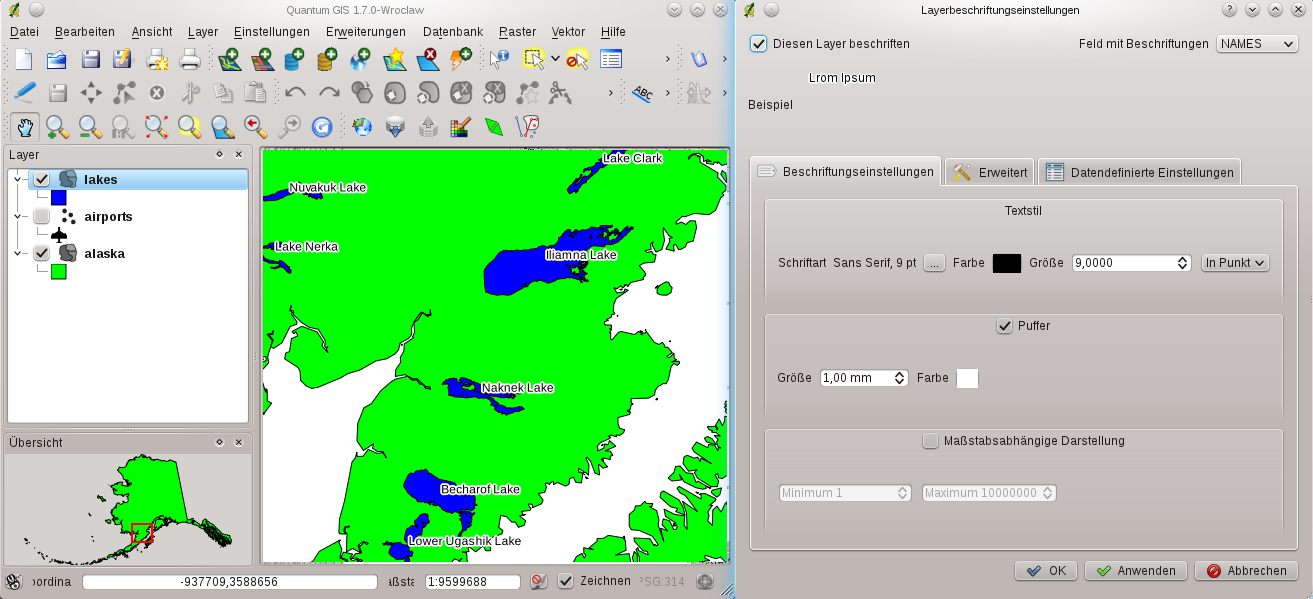
\includegraphics[clip=true, width=12cm]{label_area}
\end{center}
\end{figure}

\minisec{Change engine settings}

Additionally you can click the \button{Engine settings} button and select the search method, 
used to find the best label placement. Available is Chain, Popmusic Tabu, Popmusic Chain, 
Popmusic Tabu Chain and FALP.  

\begin{figure}[ht]
\begin{center}
   \caption{Dialog to change label engine settings \nixcaption}\label{fig:labelengine}\smallskip
   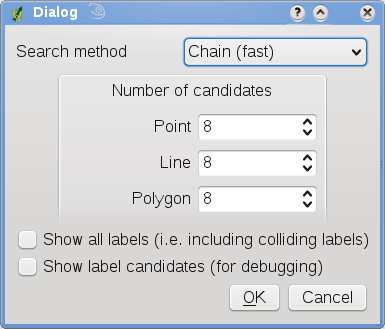
\includegraphics[clip=true, width=7cm]{label_engine}
\end{center}
\end{figure}

Furthermore the number of candidates can be defined for point, line and polygon features, 
and you can define whether to show all labels (including colliding labels) and label 
candidates for debugging.


